\section{Data source}

The National Health and Nutrition Examination Survey (NHANES) studies are a series of complex, multistage, cross-sectional surveys carried out by the National Center for Health Statistics (NCHS), which is a division of the Centers for Disease Control and Prevention. The NHANES programme is designed to assess the health and nutritional status of the non-institutionalised US population. The studies are some of the most comprehensive health surveys conducted worldwide, being unique in the detailed amount of data which is collected across the four main components: (i) health interviews, (ii) medical and dental examinations, (iii) laboratory tests, (iv) dietary interviews. The NHANES programme plays a substantial role in informing the NCHS, who use the data to publish national health statistics. The NCHS provide NHANES data open access and free-of-charge to all individuals, meaning the surveys have been used extensively in academia and policymaking for several decades \citep{cdcnhanes}.

The NHANES programme began in the early 1960s and, as of 1999, it has been carried out continuously in two-year cycles. In each cycle, a nationally representative sample of approximately 5,000 individuals are included. The data collected are then used in epidemiological studies to investigate the prevalence, determinants, and distribution of disease, as well as to direct national health policy, and a vast array of other research applications \citep{cdcnhanes}.

\section{Sampling design}

In this work, we analysed the NHANES 2017--2018 cohort. In brief, the methodologies of the NHANES studies involve interviewing participants at home and then inviting them to a mobile examination centre (MEC) for further interviews, tests, and examinations. These further tests involve an oral examination conducted by calibrated, state-licenced dental practitioners, during which the teeth, along with the presence of dental caries, restorations, missing teeth, and dental implants, are recorded. All participants are anonymised and the results of the interviews, tests, and examinations are documented as codes which were standardised across the NHANES studies \citep{bashir2022}.

The NHANES sampling methodology utilises a multi-year, stratified, clustered, four-stage design, where the data are released in two-year cycles \citep{nhanesdesign}. The sample is selected in four stages i.e., there are four levels of clustering:

\begin{enumerate}
	\item Primary sampling units (PSUs): Counties or groups of adjacent counties
	\item Secondary sampling units (SSUs): Census blocks or groups of blocks
	\item Dwelling units (DUs): Households within SSUs
	\item Individuals within DUs
\end{enumerate}

The NAHNES PSUs are selected with probabilities proportionate to size (PPS), where the measure of size (MOS) for a PSU is determined by its population count and demographics. Counties with a large enough MOS were selected with probability of 1, and these are referred to as certainty PSUs, whilst the remaining counties are known as noncertainty PSUs. Before selecting the noncertainty PSUs, the certainty PSUs were removed from the county sampling frame. The noncertainty PSUs were then stratified based on a state health index, which is a composite index based on health measures such as adult and infant mortality rates, prevalence of smoking, and prevalence of obesity. This gave rise to 14 major strata, each containing 4 minor strata, for a total of 56 minor strata. Fifteen PSUs were sampled each year; one from each major stratum plus one certainty PSU. Within each noncertainty PSU, 24 SSUs were sampled \citep{nhanesdesign}.

Some cohorts of the population were oversampled in order to increase the precision of subgroup estimates, these were \citep{nhanesdesign}: 

\begin{itemize}
	\item Those who were Hispanic
	\item Those who were Non-Hispanic Black
	\item Those who were Non-Hispanic Asian
	\item Those who were at or below 185\% of the federal poverty threshold
	\item Those who were aged 0 to 11 years, or $\geq$ 80 years
\end{itemize}

The final aspect of the NHANES design was computation of survey weights. The survey weights account for various aspects of the survey design \citep{nhanesdesign}:

\begin{itemize}
	\item Probability of selection
	\item Differential rates of nonresponse at each level of data collection (i.e., screening, interview, examination)
	\item Discrepancy between the distribution of the sample and target population
\end{itemize}

The weights were then calibrated by a process known as poststratification. This adjusts the weights to account for under- or over-coverage of certain demographic subgroups, as well as differential rates of nonresponse within each of these subgroups. Known population totals for age-sex-race-ethnicity-income-education subgroups were obtained from the 2017 American Community Survey (ACS). The weights were then adjusted so that the weighted survey counts matched the population counts in the 2017 ACS \citep{nhanesdesign}. Given that nonresponse rates differed at the interview, examination, and laboratory testing stages, a different set of survey weights were calculated for each of these stages. Depending on the data analysed, the appropriate survey weights must be used in a "lowest common denominator" fashion. For example, if all data analysed were collected at the interview stage only, then the interview survey weights should be used. If data were from a combination of the interview and examination stages, then the MEC survey weights should be used.

\section{Inclusion criteria}

We specified the following inclusion criteria: participants aged between 2 to 11 years, who had undergone a complete oral examination, with data recorded on country of birth and sociodemographics. The full details of how the NHANES 2017--2018 cohort were processed prior to analysis are presented in \autoref{fig:strobe-flowchart}.

\begin{figure}[ht]
\centering
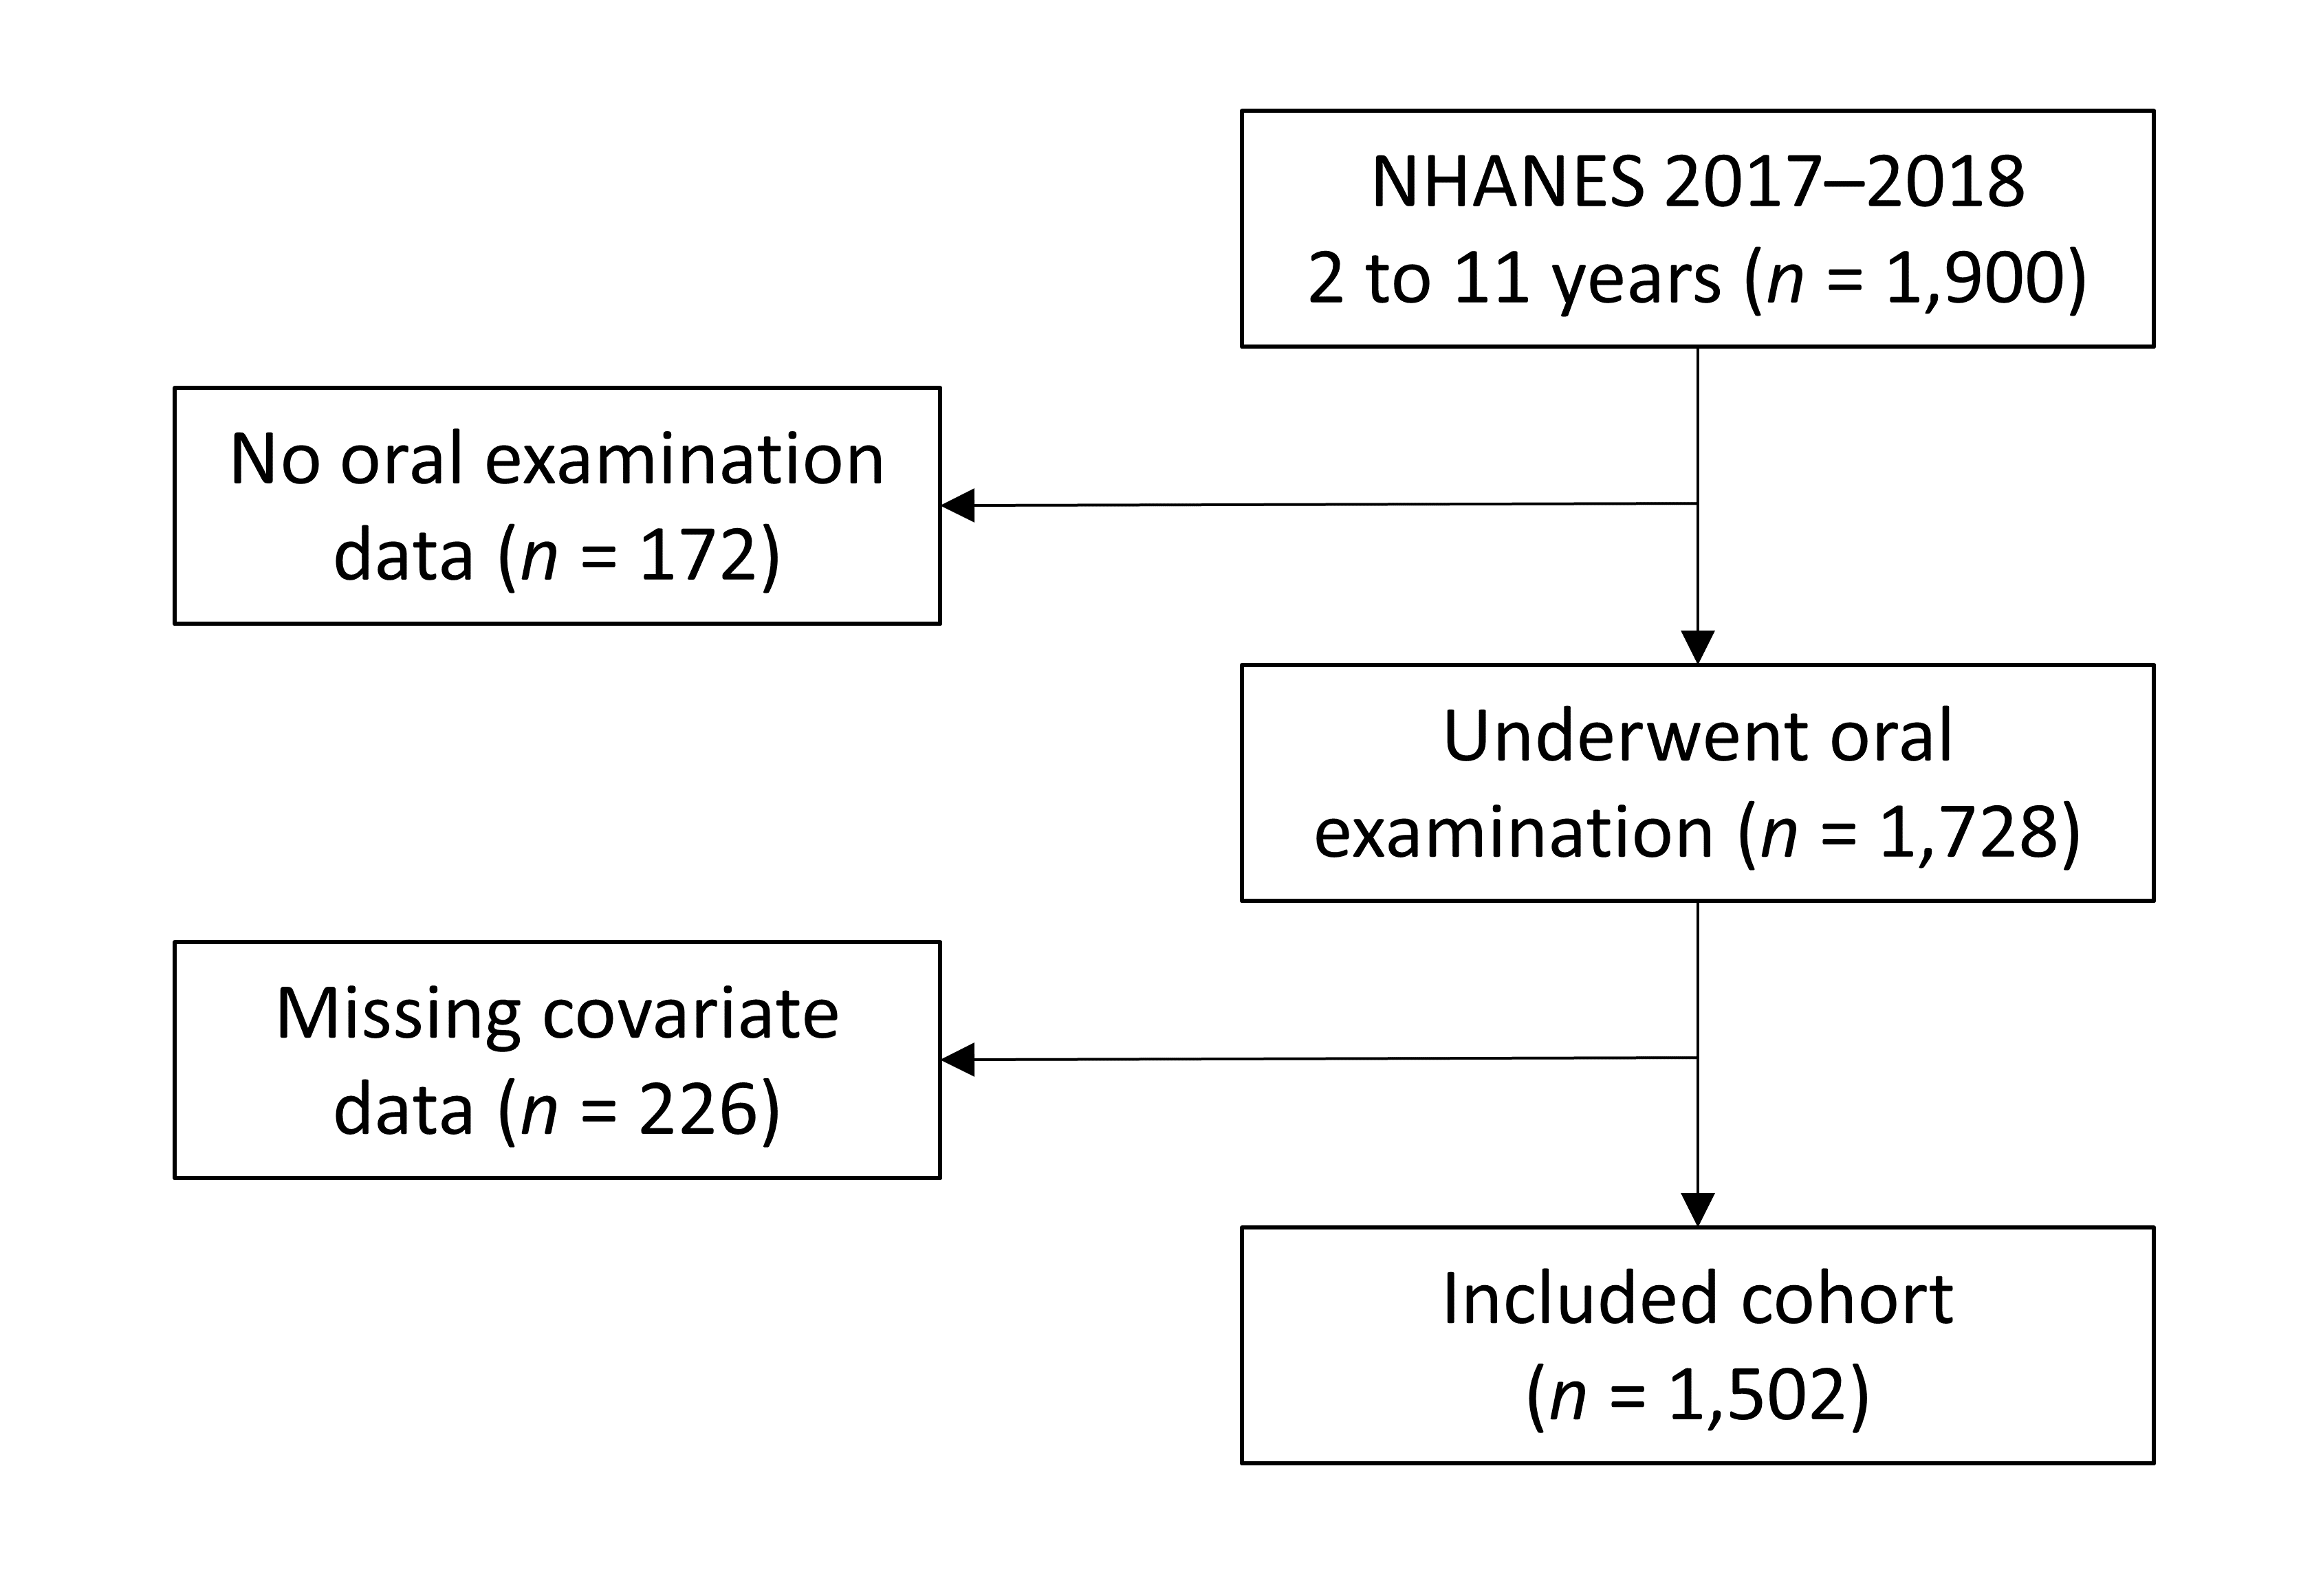
\includegraphics[scale = 0.8]{images/strobe}
\caption{Flowchart illustrating processing of the NHANES 2017--2018 cohort.}
\label{fig:strobe-flowchart}
\end{figure}

\section{Variables}

\subsection{Outcome}

The outcome of interest was the presence or absence of dental caries. Participants were defined as having dental caries if any tooth in the mouth had an active carious lesion, where the diagnostic criteria for dental caries were those developed by \citet{radike1968}. Namely, these were the presence of any of the following features: gross cavitation; a deep pit or fissure with either softness at the base of the area or an opacity adjacent to the area providing evidence of undermining or demineralization; white spots or subsurface demineralization found to be soft on probing with the explorer; proximal caries as diagnosed using the same criteria for deep pits, fissures, or smooth surfaces; the presence of breaks in the enamel or subsurface shadowing on the proximal surfaces of teeth; and loss of translucency identified via transillumination on proximal surfaces of anterior teeth only. The presence of caries on the root surfaces was not assessed in participants below the age of 18 years \citep{bashir2022}.

Briefly, the caries assessment component of the oral examination involved rinsing out the mouth before examination, removal of food debris with 2$\times$2 inch sponges, and examination of all teeth except third molars using visual and tactile feedback from a no. 23 explorer, hand mirror, and lighting. The teeth were examined in a standardized order for each participant, and trained health technicians documented the presence of dental caries, and the surfaces affected \citep{bashir2022}.

\subsection{Exposure}

The exposure of interest was nativity status. Individuals were asked in which country they were born: if they replied that they were born in one of the 50 US states or Washington, DC, then they were classified as being US-native (i.e., non-migrants), whereas if they replied that they were born outside of the US they were classified as being non-US-native (i.e., migrants).

\subsection{Covariates}

The covariates of interest were: 

\begin{itemize}
	\item Age: Continuous variable measured in years
	\item Sex: Categorical variable taking values \{Male, Female\}
	\item Race/ethnicity: Categorical variable taking values \{Non-Hispanic White, Non-Hispanic Black, Hispanic, Non-Hispanic Asian, Other\}
	\item Household education: Categorical variable taking values \{Below high school, High school graduate, College (i.e., university) graduate\}
	\item Family income-to-poverty ratio (FIPR): Continuous variable defined as the ratio between household income and the federal poverty threshold i.e., FIPR < 100\% indicates an income below the federal poverty threshold
\end{itemize}

Household education was defined as the maximum level of education attained by the household reference person. The household reference person is defined in NHANES as the first household member 18 years of age or older, who owns or rents the residence where members of the household reside \citep{nhanesdemo}. Demographic information pertaining to the reference person acts as a marker of socioeconomic status for the household being surveyed.

\section{Statistical analysis}

All analyses were designed and reported according to the Strengthening the Reporting of Observational Studies in Epidemiology (STROBE) guidelines \citep{strobe}.

\subsection{Descriptive analyses}

We computed summary statistics for the included cohort, including the number of observations, the represented population, means and proportions, and the design effects. The represented population is the number of individuals in the target population who are represented by the sample, where the target population in this case is the US paediatric population aged between 2 to 11 years. We also computed summary statistics stratified by the presence or absence of dental caries, and then tested for differences between individuals with and without disease using a design-adjusted \emph{t}-test for continuous variables and a Rao-Scott \emph{F}-test for categorical variables. The Rao-Scott \emph{F}-test is a Pearson $\chi^{2}$ test which is adjusted for the complex survey design by applying the second-order correction described by \citet{rao1984}, and then converted into an \emph{F}-statistic.

\subsection{Model fitting}

We fit a logistic regression model to test for the association between nativity status and risk of dental caries using the incremental model building process specified by \citet{hosmer2000}:

\begin{enumerate}
	\item Carry out bivariate tests of association between the outcome and predictors
	\item Include the predictors which have bivariate association with the outcome at a significance level of $p < 0.25$ as main effects in a logistic regression model
	\item Assess the association of each predictor with the outcome using the Wald test
	\item Compare each of the coefficients in the multivariable model with the coefficients from a univariable model (i.e., a model containing only that variable)
	\item Evaluate scientifically justified interactions between the predictors
\end{enumerate}

In addition to the above, we did the following:

\begin{itemize}
	\item We carried out a Wald test on the multivariable model testing the null hypothesis that all parameters were simultaneously equal to 0
	\item We carried out a PLRT on the multivariable model testing the null hypothesis that the model does not fit better than the null model
	\item For each univariable model, we carried out a Wald test to assess how the variable was associated with the outcome, without adjusting for confounders
	\item We computed the weighted AUCROC for the multivariable model
	\item We computed the design effects for the parameter estimates in the multivariable model
\end{itemize}

All analyses were conducted in line with the CDC guidelines for analysing NHANES data and adjustment for the CSS design was made by using the MEC-specific sampling weights, as well as the cluster- and stratum-identifying variables.